%%%%%%%%%%%%%%%%%%%%%%%%%%%%%%%%%%%%%%%%%
% Short Sectioned Assignment
% LaTeX Template
% Version 1.0 (5/5/12)
%
% This template has been downloaded from:
% http://www.LaTeXTemplates.com
%
% Original author:
% Frits Wenneker (http://www.howtotex.com)
%
% License:
% CC BY-NC-SA 3.0 (http://creativecommons.org/licenses/by-nc-sa/3.0/)
%
%%%%%%%%%%%%%%%%%%%%%%%%%%%%%%%%%%%%%%%%%

%----------------------------------------------------------------------------------------
%	PACKAGES AND OTHER DOCUMENT CONFIGURATIONS
%----------------------------------------------------------------------------------------

\documentclass[paper=a4, fontsize=11pt]{scrartcl} % A4 paper and 11pt font size

\usepackage[T1]{fontenc} % Use 8-bit encoding that has 256 glyphs
%\usepackage{fourier} % Use the Adobe Utopia font for the document - comment this line to return to the LaTeX default
\usepackage[english]{babel} % English language/hyphenation
\usepackage{amsmath,amsfonts,amsthm} % Math packages
\usepackage[utf8]{inputenc}
\usepackage{lipsum} % Used for inserting dummy 'Lorem ipsum' text into the template

\usepackage{sectsty} % Allows customizing section commands
\allsectionsfont{\centering \normalfont\scshape} % Make all sections centered, the default font and small caps

\usepackage{fancyhdr} % Custom headers and footers
\usepackage{listings}
\usepackage{graphicx}


\pagestyle{fancyplain} % Makes all pages in the document conform to the custom headers and footers
\fancyhead{} % No page header - if you want one, create it in the same way as the footers below
\fancyfoot[L]{} % Empty left footer
\fancyfoot[C]{} % Empty center footer
\fancyfoot[R]{\thepage} % Page numbering for right footer
\renewcommand{\headrulewidth}{0pt} % Remove header underlines
\renewcommand{\footrulewidth}{0pt} % Remove footer underlines
\setlength{\headheight}{13.6pt} % Customize the height of the header

\numberwithin{equation}{section} % Number equations within sections (i.e. 1.1, 1.2, 2.1, 2.2 instead of 1, 2, 3, 4)
\numberwithin{figure}{section} % Number figures within sections (i.e. 1.1, 1.2, 2.1, 2.2 instead of 1, 2, 3, 4)
\numberwithin{table}{section} % Number tables within sections (i.e. 1.1, 1.2, 2.1, 2.2 instead of 1, 2, 3, 4)

\setlength\parindent{0pt} % Removes all indentation from paragraphs - comment this line for an assignment with lots of text

%----------------------------------------------------------------------------------------
%	TITLE SECTION
%----------------------------------------------------------------------------------------

\newcommand{\horrule}[1]{\rule{\linewidth}{#1}} % Create horizontal rule command with 1 argument of height
\newcommand{\norm}[1]{\left\lVert#1\right\rVert}

\title{	
\normalfont \normalsize 
\textsc{University of Helsinki, Department of Computer Science} \\ [25pt] % Your university, school and/or department name(s)
\horrule{0.5pt} \\[0.4cm] % Thin top horizontal rule
\huge Assignment 2 of Introduction to Machine Learning \\ % The assignment title
\horrule{2pt} \\[0.5cm] % Thick bottom horizontal rule
}

\author{Gao Yuan No.014242582} % Your name

\date{\normalsize\today} % Today's date or a custom date

\begin{document}

\maketitle % Print the title

%----------------------------------------------------------------------------------------
%	PROBLEM 1
%----------------------------------------------------------------------------------------

\section{Problem 1}
Answer:
\newline
As the logarithmic model is proper, we use logarithmic cost function for evaluation.
\begin{figure}[h!]
  \centering
    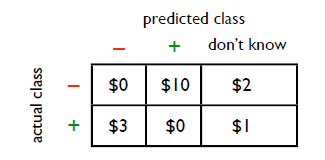
\includegraphics[width=0.5\textwidth]{problem_1_figure}
      \caption{Confusion matrix of KNN classifier.}
\end{figure}
We assume the probability of assigning to first class is $p$ then the probability of assigning second class is $1-p$.


The expected cost would be 
\begin{align}
E\{'-'\} &=  0(1-\alpha) + 3\alpha 
\end{align}
\begin{align}
E\{'+'\} &=  10(1-\alpha) + 0\alpha 
\end{align}
\begin{align}
E\{'don't know'\} &=  2(1-\alpha) + 1\alpha
\end{align}

\begin{align}
E\{'-'\} &= E\{'+'\} \\
0(1-\alpha) + 3\alpha  &=  10(1-\alpha) + 0\alpha  \\
\alpha_1 & = \frac{10}{13}
\end{align}
\begin{align}
E\{'-'\} &= E\{'don't know'\} \\
0(1-\alpha) + 3\alpha  &= 2(1-\alpha) + 1\alpha \\
\alpha_2 & = \frac{1}{2}
\end{align}
\begin{align}
E\{'+'\} &= E\{'don't know'\} \\
10(1-\alpha) + 0\alpha  &= 2(1-\alpha) + 1\alpha \\
\alpha_3 & = \frac{8}{9}
\end{align}

The best answer for '-','+' and 'don't know' are that:

\begin{itemize}
  \item When $\alpha$ is smaller or equal to $\frac{1}{2}$, we predict '-'.
  \item When $\alpha$ is bigger than $\frac{1}{2}$ and $\alpha$ is smaller or equal to $\frac{8}{9}$, we predict 'don't know'.
  \item When $\alpha$ is bigger than $\frac{8}{9}$, we predict '+'.
\end{itemize}
%------------------------------------------------

\section{Problem 2}
Answer:
\newline
\newline
The expected cost is:
\begin{align}
E\{C\} &= E\{1\} + E\{0\}\\
&=  (b-1)^2 a + b^2(1-a) \\
&=  b^2a-2ba+a + b^2 - b^2a \\
&= -2ba + a + b^2 
\end{align}
First order derivative is :
\begin{align}
\frac{\partial E\{C\}}{\partial b} &=  \frac{\partial (-2ba + a + b^2)}{\partial b} \\
&= -2a + 2b
\end{align}
Second order derivative is :
\begin{align}
\frac{\partial (-2a + 2b)}{\partial b} &=  2  \\
&\geq 0
\end{align}
As a consequence, $E\{C\}$ is minimized, when $-2a + 2b = 0$ (i.e. when $a = b $).
\newline
\newline
\section{Problem 3}
Proximity is typically defined between a pair of objects.
\newline
\newline
For class $P(y = 0) = 0.2$, there are $2 \times 3 = 6 $ unit areas. For class $P(y = 1) = 0.7$, there are $4 \times 4 = 16 $ unit areas. For class $P(y = 2) = 0.1$, there are $3 \times 3 = 9 $ unit areas. The proportionality of possibility of these three areas are $\frac{0.2}{6}$,$\frac{0.7}{16}$ and $\frac{0.1}{9}$ respectively.
\newline
\newline
\newline
$X_1$ is located in the area of $y = 0, y = 1$ and $y = 2$, the normalized possibilities of being in categories are as follows: 
\begin{table}[!htbp]
\centering
\begin{tabular}{|c|c|c|}
\hline 
$y = 0$ & $y = 1$ & $y = 2$ \\ 
\hline 
0 & 1 & 0 \\ 
\hline 
\end{tabular} 
\end{table}


$X_2$ is located in the area of $y = 0, y = 1$ and $y = 2$, the normalized possibilities of being in categories are as follows: 
\begin{table}[!htbp]
\centering
\begin{tabular}{|c|c|c|}
\hline 
$y = 0$ & $y = 1$ & $y = 2$ \\ 
\hline 
0.3780 & 0.4961 & 0.1260. \\ 
\hline 
\end{tabular} 
\end{table}

$X_3$ is located in the area of $y = 1$ and $ y = 2$, the normalized possibility of being in categories $y = 0, y = 1$ and $y = 2$ are 0, 0.7975 and 0.2025.
\begin{table}[!htbp]
\centering
\begin{tabular}{|c|c|c|}
\hline 
$y = 0$ & $y = 1$ & $y = 2$ \\ 
\hline 
0 & 0.7975 & 0.2025. \\ 
\hline 
\end{tabular} 
\end{table}
\newline
$X_4$ is located in the area of $y = 0$ and $ y = 2$,, the normalized possibility of being in categories $y = 0, y = 1$ and $y = 2$ are 0.75, 0, 0.25 .
\begin{table}[!htbp]
\centering
\begin{tabular}{|c|c|c|}
\hline 
$y = 0$ & $y = 1$ & $y = 2$ \\ 
\hline 
0.75 & 0 & 0.25. \\ 
\hline 
\end{tabular} 
\end{table}
\newline
$X_5$ is located in the area of $y = 2$, the normalized possibility of being in categories $y = 0, y = 1$ and $y = 2$ are 0, 0, 1.
\begin{table}[!htbp]
\centering
\begin{tabular}{|c|c|c|}
\hline 
$y = 0$ & $y = 1$ & $y = 2$ \\ 
\hline 
0 & 0 & 1 \\ 
\hline 
\end{tabular} 
\end{table}
\section{Problem 4}

(a) Download the MNIST data from the course web page. In addition to the actual data, the package con-tains some functions for easily loading the data into Matlab/Octave/R and for displaying digits. See the README files for details. Load the rst N=5,000 images using the provided function.
\newline
\newline
Answer:
\newline\begin{figure}[h!]
  \centering
    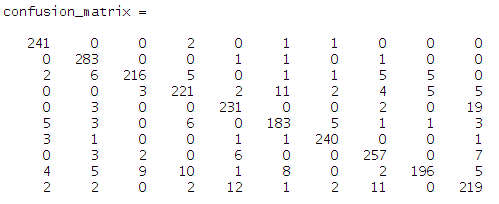
\includegraphics[width=0.8\textwidth]{confusion_matrix_knn}
      \caption{Confusion matrix of KNN classifier.}
\end{figure}
done !
\newline
\newline
(b) Use the provided functions to plot a random sample of 100 handwritten digits, and show the associated
labels. Verify that the labels match the digit images. (This is a sanity check that you have the data is in
the right format.)
\newline
\newline
Answer:
\newline
The code past the sanity test.
\newline
\newline
(c) Divide the data into two parts: A `training set' consisting of the rst 2,500 images (and associated labels),and a `test set' containing the remaining 2,500 images (and their associated labels).
\newline
\newline
Answer:
\newline
The following code has been used for dividing training set and test set.
\begin{lstlisting}
 first_part= 1:N/2;
 second_part = 1:N;
 second_part = setdiff(second_part,first_part);
\end{lstlisting}

(d) For each of the ten classes (digits 0-9), compute a class prototype given by the mean of all the images in
the training set that belong to this class. That is, select from the training set all images of class `0' and
compute the mean image of these; this should look sort of like a zero. Do this for all ten classes, and plot
the resulting images. Do they look like what you would expect?
\newline
\newline
Answer:
\newline
They do look like the same as the average of each digit.
\newline
\newline
(e) For each of the images in the test set, compute the Euclidean distance of the image to all 10 prototypes,
and classify the test image into the class for which the distance to the prototype is the smallest. So, if a
test image is closer to the prototype for `3' than it is to the prototypes for any of the other digits, predict
its class to be `3'. Compute and display the resulting confusion matrix.
\newline
Answer:
\newline
The confusion matrix is as follows.
\begin{figure}[h!]

  \centering
    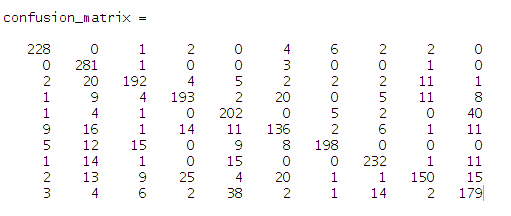
\includegraphics[width=0.8\textwidth]{confusion_matrix_edulean_dis}
      \caption{Confusion matrix of edulean classifier.}
\end{figure}
\newline
\newline
(f) Classify each of the test images with a nearest neighbor classifer: For each of the test images, compute
its Euclidean distance to all (2,500) of the training images, and let the predicted class be the class of the
closest training image. Compute and display the resulting confusion matrix.
\newline
Answer:
\newline
The confusion matrix is as follows.
\begin{figure}[h!]
  \centering
    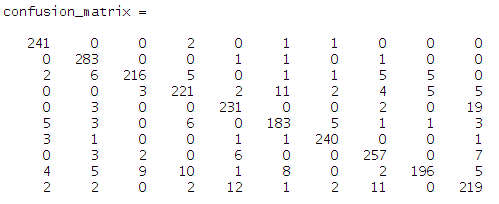
\includegraphics[width=0.8\textwidth]{confusion_matrix_knn}
      \caption{Confusion matrix of KNN classifier.}
\end{figure}
\newline
\newline
(g) Compute and compare the error rates of both classi ers (the prototype-based classi er and the nearestneighbor classi er). Which is working better? Based on the confusion matrix, which digits are confusedwith each other? Why do you think this is?
\newline
Answer:
\newline
1) The error rate of edulean distance classifier is 0.2036 and the error rate of NN is 0.0852. 
\newline
2) The NN classifier is working better.
\newline
3) 5 and 9 are the most confusing digits.
\newline
4) The shapes of these two digits are the similar in many cases.
\end{document}

